%%%% Modèle proposé par kira.ribeiro@universite-paris-saclay.fr %%%%
%%%% màj : 29 octobre 2021 %%%%

\documentclass[french,12pt,a4paper]{book}
\usepackage[utf8]{inputenc}
\usepackage[T1]{fontenc}
\usepackage[french]{babel}
\usepackage[default,oldstyle, scale=.95]{opensans} % police Open Sans
\usepackage{amsmath}
\usepackage{amsfonts}
\usepackage{fancyhdr}
\usepackage{amssymb}
\usepackage{xcolor} % où color selon l'installation
\definecolor{Prune}{RGB}{99,0,60} % l14-33 : couleurs de la charte graphique upsaclay
\definecolor{B1}{RGB}{49,62,72} 
\definecolor{C1}{RGB}{124,135,143}
\definecolor{D1}{RGB}{213,218,223}
\definecolor{A2}{RGB}{198,11,70}
\definecolor{B2}{RGB}{237,20,91}
\definecolor{C2}{RGB}{238,52,35}
\definecolor{D2}{RGB}{243,115,32}
\definecolor{A3}{RGB}{124,42,144}
\definecolor{B3}{RGB}{125,106,175}
\definecolor{C3}{RGB}{198,103,29}
\definecolor{D3}{RGB}{254,188,24}
\definecolor{A4}{RGB}{0,78,125}
\definecolor{B4}{RGB}{14,135,201}
\definecolor{C4}{RGB}{0,148,181}
\definecolor{D4}{RGB}{70,195,210}
\definecolor{A5}{RGB}{0,128,122}
\definecolor{B5}{RGB}{64,183,105}
\definecolor{C5}{RGB}{140,198,62}
\definecolor{D5}{RGB}{213,223,61}
\usepackage{mdframed}
\usepackage{multirow} %% Pour mettre un texte sur plusieurs rangées
\usepackage{multicol} %% Pour mettre un texte sur plusieurs colonnes
\usepackage{tikz}
\usepackage{graphicx}
\usepackage[absolute]{textpos} 
\usepackage{colortbl}
\usepackage{array}
\usepackage{geometry}
\usepackage{titlesec}
\usepackage{hyperref}
\hypersetup{ % paramétrage couleur des liens hypertextes, toujours garder colorlinks=true
    colorlinks=true,
    linkcolor=black,
    urlcolor=purple}


\pagestyle{plain} % pour ne garder que les n°de page en milieu-bas et supprimer les indications de chapitre en marge haute

\usepackage{lipsum} % à retirer!!!
\begin{document}

\begin{titlepage}

%\thispagestyle{empty}

\newgeometry{left=6cm,bottom=2cm, top=1cm, right=1cm}

\tikz[remember picture,overlay] \node[opacity=1,inner sep=0pt] at (-13mm,-135mm){
\includegraphics{Frame-ups.pdf}};

%*****************************************************
%******** NUMÉRO D'ORDRE DE LA THÈSE À COMPLÉTER *****
%******** POUR LE SECOND DÉPOT                   *****
%*****************************************************

\color{white}

\begin{picture}(0,0)
\put(-152,-743){\rotatebox{90}{\Large \textsc{THESE DE DOCTORAT}}} \\
\put(-120,-743){\rotatebox{90}{NNT : 2020UPASA001}}
\end{picture}
 
%*****************************************************
%**  LOGO  ÉTABLISSEMENT PARTENAIRE SI COTUTELLE
%**  CHANGER L'IMAGE PAR DÉFAUT **
%*****************************************************
\vspace{-14mm} % à ajuster en fonction de la hauteur du logo
\flushright 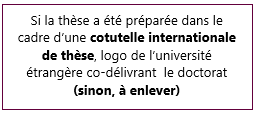
\includegraphics[scale=1]{logo2.png}

%*****************************************************
%******************** TITRE **************************
%*****************************************************

\flushright
\vspace{10mm} % à régler éventuellement
\color{Prune}
\fontfamily{cmss}\fontseries{m}\fontsize{22}{26}\selectfont
  \Huge Titre de la thèse (sur plusieurs lignes si nécessaire) \\

\normalsize
\color{black}
\Large{\textit{Traduction du titre de la thèse (sur plusieurs lignes si nécessaire)}} \\
%*****************************************************

\fontfamily{fvs}\fontseries{m}\fontsize{8}{12}\selectfont

\vspace{1.5cm}

\normalsize
\textbf{Thèse de doctorat de l'université Paris-Saclay et de l'université XXX (si cotutelle - sinon enlever cette seconde partie)} \\

\vspace{6mm}

\small École doctorale n$^{\circ}$ d'accréditation, dénomination et sigle\\
\small Spécialité de doctorat: voir annexe\\
\small Graduate School : voir annexe. Référent : voir annexe \\
\vspace{6mm}

\footnotesize Thèse préparée dans la (ou les) unité(s) de recherche \textbf{Nom(s)} (voir annexe), sous la direction de \textbf{Prénom NOM}, titre du directeur ou de la directrice de thèse, la co-direction de \textbf{Prénom NOM}, titre du co-directeur ou de la co-directrice de thèse, le co-encadrement de \textbf{Prénom NOM}, titre, du co-encadrant ou de la co-encadrante ou la co-supervision de \textbf{Prénom NOM}, titre, du tuteur ou de la tutrice (en cas de partenariat industriel) \\
\vspace{15mm}

\textbf{Thèse soutenue à Paris-Saclay, le JJ mois AAAA, par}\\
\bigskip
\Large {\color{Prune} \textbf{Prénom NOM}} % Changer le Prénom et le NOM

%************************************
\vspace{\fill} % ALIGNER LE TABLEAU EN BAS DE PAGE
%************************************

\bigskip

\flushleft
\small {\color{Prune} \textbf{Composition du jury}}\\
{\color{Prune} \scriptsize {Membres du jury avec voix délibérative}} \\
\vspace{2mm}
\scriptsize
\begin{tabular}{|p{7cm}l}
\arrayrulecolor{Prune}
\textbf{Prénom NOM} &   Président ou Présidente\\ 
Titre, Affiliation & \\
\textbf{Prénom NOM} &  Rapporteur \& Examinateur / trice \\ 
Titre, Affiliation   &   \\ 
\textbf{Prénom NOM} &  Rapporteur \& Examinateur / trice \\ 
Titre, Affiliation  &   \\ 
\textbf{Prénom NOM} &  Examinateur ou Examinatrice \\ 
Titre, Affiliation   &   \\ 
\textbf{Prénom NOM} &  Examinateur ou Examinatrice \\ 
Titre, Affiliation   &   \\ 
 

\end{tabular} 

\end{titlepage}


% page des résumés à garder en 2ème page. Si les résumés sont trop longs pour tenir sur une seule et même page, on peut mettre un résumé par page
\thispagestyle{empty}
\newgeometry{top=1.5cm, bottom=1.25cm, left=2cm, right=2cm}
\fontfamily{rm}\selectfont

\lhead{}
\rhead{}
\rfoot{}
\cfoot{}
\lfoot{}

\noindent 
%*****************************************************
%***** LOGO DE L'ED À CHANGER IMPÉRATIVEMENT *********
%*****************************************************
\includegraphics[height=2.45cm]{logo_ups_EOBE.png}
\vspace{1cm}
%*****************************************************
\fontfamily{cmss}\fontseries{m}\selectfont

\small

\begin{mdframed}[linecolor=Prune,linewidth=1]

\textbf{Titre:} titre (en français)..................................................................................................................

\noindent \textbf{Mots clés:} 3 à 6 mots clefs (version en français)

\vspace{-.5cm}
\begin{multicols}{2}
\noindent \textbf{Résumé:}\lipsum[1-2] 
\end{multicols}

\end{mdframed}

\vspace{8mm}

\begin{mdframed}[linecolor=Prune,linewidth=1]

\textbf{Title:} titre (en anglais)..................................................................................................................

\noindent \textbf{Keywords:} 3 à 6 mots clefs (version en anglais)

\begin{multicols}{2}
\noindent \textbf{Abstract:} \lipsum[1-2]
\end{multicols}
\end{mdframed}

\titleformat{\chapter}[hang]{\bfseries\Large\color{Prune}}{\thechapter\ -}{.1ex}
{\vspace{0.1ex}
}
[\vspace{1ex}]
\titlespacing{\chapter}{0pc}{0ex}{0.5pc}

\titleformat{\section}[hang]{\bfseries\normalsize}{\thesection\ .}{0.5pt}
{\vspace{0.1ex}
}
[\vspace{0.1ex}]
\titlespacing{\section}{1.5pc}{4ex plus .1ex minus .2ex}{.8pc}

\titleformat{\subsection}[hang]{\bfseries\small}{\thesubsection\ .}{1pt}
{\vspace{0.1ex}
}
[\vspace{0.1ex}]
\titlespacing{\subsection}{3pc}{2ex plus .1ex minus .2ex}{.1pc}

\newgeometry{top=4cm, bottom=4cm, left=2cm, right=2cm}

\tableofcontents

\newgeometry{top=4cm, bottom=4cm, left=4cm, right=4cm}

\chapter{AVERTISSEMENT}
La composition de la page de couverture doit être respectée pour la diffusion de la thèse sur \url{www.theses.fr} et pour le dépôt légal de la thèse, qui est obligatoire pour l’obtention du diplôme (\href{https://www.legifrance.gouv.fr/affichTexte.do?cidTexte=JORFTEXT000032587086&dateTexte=20160902}{cf. articles 24 et 25 de l’arrêté du 25 mai 2016 fixant le cadre national de la formation et les modalités conduisant à la délivrance du diplôme national de doctorat}).\\ \par
Les consignes et les recommandations ci-après ont pour objet d’assurer une \textbf{homogénéité graphique} pour toutes les thèses soutenues à l’université Paris-Saclay et de les rendre \textbf{immédiatement reconnaissables}.\\ \par
Elles ont également pour objet de donner un cadre de référence permettant d’éviter qu’un lecteur futur puisse avoir des \textbf{doutes sur la conformité de la thèse ou du jury}. L’université reçoit régulièrement des demandes d’informations, au sujet de thèses, pour lesquelles il y a des questionnements sur la conformité du jury ou bien des incohérences entre les informations qui figurent sur la couverture de la thèse, d’une part, et les méta-données de la thèse visibles sur www.theses.fr, d’autre part.\\ \par
Il est rappelé que ces consignes et recommandations ne s’appliquent que pour le dépôt légal de la thèse et sa diffusion via le portail \url{www.theses.fr}. \textbf{Ce canal de diffusion n’est pas exclusif}. D’autres formats de page de couverture peuvent être librement utilisés par les auteurs sur d’autres canaux de diffusion (par exemple : pour afficher le nom et le logo d’une organisation qui aurait co-financé la thèse et pour la diffusion au sein de cette organisation), à condition que les informations requises pour la citation complète de la thèse de doctorat figurent. C’est-à-dire : au minimum : nom et prénom de l’auteur, titre de la thèse, date, lieu et établissement de soutenance (université Paris-Saclay et le cas échéant un établissement partenaire en cas de cotutelle internationale de thèse), ainsi que le logo de l’université Paris-Saclay et le cas échéant d’une université étrangère partenaire en cas de cotutelle internationale de thèse.

\chapter{COMPOSITION GÉNÉRALE, CHARTE GRAPHIQUE}
\section{COMPOSITION DU DOCUMENT}
Les deux premières pages sont consacrées aux informations institutionnelles. \\ \par
Une troisième page peut être ajoutée pour compléter les informations institutionnelles réglementaires des deux premières pages. Par exemple, pour donner des informations sur l’organisme d’accueil ou financeur et afficher leurs logos, pour décrire brièvement un cadre partenarial, pour fournir les noms de personnalités invitées à siéger aux cotés du Jury pour la soutenance, pour afficher le logo du laboratoire etc. \\ \par 
La page des remerciements est alors placée en 3\ieme ou 4\ieme page, selon qu’une 3\ieme page a été ajoutée ou non pour apporter ces compléments d’informations.
\section{QUELS LOGOS FAIRE FIGURER ?}
Il ne doit figurer sur la \textbf{page de couverture de thèse}, aucun autre logo que le \textbf{logo de l’université Paris-Saclay} et, en cas de cotutelle internationale de thèse, le logo de l’université partenaire étrangère qui délivre également le diplôme de doctorat pour cette thèse. \\ \par
Il ne doit figurer sur la \textbf{seconde page}, aucun autre logo que le \textbf{logo de l’école doctorale}.
Les logos institutionnels en vigueur de l’université Paris-Saclay et des écoles doctorales sont fournis au paragraphe 7.2.\\ \par
Les autres logos, comme celui du laboratoire, d’une entreprise, d’une composante, d’un établissement-composante, d’une université membre associée, d’un organisme de recherche ou de toute autre organisation partenaire de la thèse, peuvent être regroupés dans une troisième page intérieure, avant la page des remerciements, mais ne doivent pas figurer pas sur les deux premières pages.
\section{POLICES DE CARACTÈRES ET COULEURS}
Les polices de caractère à utiliser sont : Open Sans ou Segoe UI ou Tahoma ou Ebrima. Il ne faut utiliser qu’\textbf{une seule police de caractère}.\\ \par
Sur les 3 premières pages, seules deux couleurs de police sont utilisées, noir et prune (R : 99 V : 0 B : 60). Dans le reste du document, vous pouvez utiliser d’autres couleurs de police, si nécessaire, en veillant à ce qu’elles appartiennent à la palette de couleurs de la charte graphique de l’université Paris-Saclay.  D’autres nuances de couleurs peuvent être utilisées parmi les nuances de la palette de l’UPSaclay.\\ \par

\begin{center} 
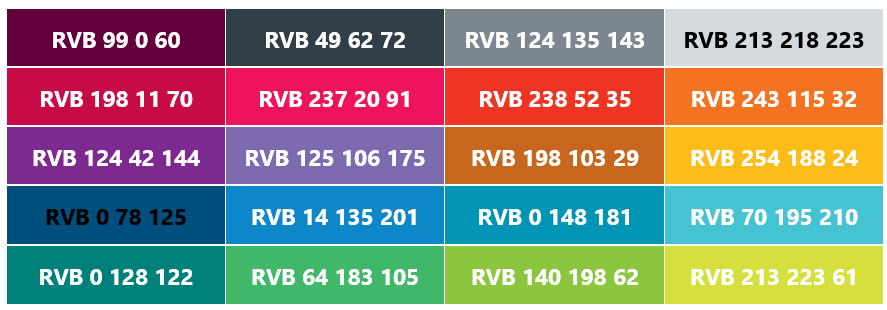
\includegraphics[scale=0.6]{Charte_graphique_ups.png}
\end{center}

La \href{https://portail.universite-paris-saclay.fr/communication/Pages/Charte-graphique.aspx}{charte graphique de l’Université} peut être téléchargée sur l’intranet pour plus d’information.\\ \par
Sur la couverture de la thèse, le \textbf{titre} est en police normale de taille 20, de couleur prune et la \textbf{traduction du titre} est en police normale de taille 12, de couleur noire et en italique. Si le titre et sa traduction sont très longs, la police peut éventuellement être réduite, mais sans descendre en dessous d’une police 14 pour le titre et d’une police 10 pour la traduction du titre.

\chapter{INFORMATIONS GÉNÉRALES SUR LA PAGE DE COUVERTURE}
Les informations figurant sur la page de couverture de la thèse doivent être cohérentes avec le diplôme et avec les métadonnées de la thèse sur le portail nationale des thèses \url{www.theses.fr}.
\section{TITRE DE LA THÈSE ET LANGUE(S)}
Le \textbf{titre de la thèse} doit être fourni en \textbf{français} et en \textbf{anglais}. Par défaut, le titre est en français et la traduction du titre est en anglais. Cependant, lorsque la thèse est rédigée en anglais, le titre peut être fourni en anglais et la traduction en français.\\ \par
Les affiliations (université de rattachement…) peuvent, le cas échéant, être fournies en anglais pour des membres étrangers du Jury. La langue par défaut restant le français.\\ \par
Tous les autres éléments de la couverture de la thèse sont en français, les noms des entités (école doctorale, unité de recherche, référent etc.) ainsi que les titres des membres du jury (Professeur, Maître de Conférences etc.). Les correspondances entre titres étrangers et français peuvent être trouvées sur le site du ministère (\href{https://www.galaxie.enseignementsup-recherche.gouv.fr/ensup/pdf/EC_pays_etrangers/Tableau_comparaison_au_26_septembre_2012.pdf}{GALAXIE})\footnote{\url{https://www.galaxie.enseignementsup-recherche.gouv.fr/ensup/pdf/EC_pays_etrangers/Tableau_comparaison_au_26_septembre_2012.pdf}}.
\section{SPÉCIALITÉ DE DOCTORAT}
La spécialité de doctorat doit faire partie des spécialités pour lesquelles l’école doctorale est accréditée (en pratique : cela implique que vous devez pouvoir la sélectionner dans le menu déroulant des spécialités dans Adum). \\ \par
La spécialité de doctorat retenue, via le menu déroulant dans Adum, sera celle qui figurera sur le diplôme.\\ \par
Si votre spécialité n’apparaît pas, il faut contacter le directeur de votre école doctorale.
\newpage
\section{UNITÉ DE RECHERCHE}
L’unité de recherche dans laquelle la thèse a été préparée est précisée sur la couverture de la thèse. Le nom de l’unité est cité en respectant les règles de signature officielles, telles qu’elles ont été convenues entre les tutelles des unités de recherche liées à l’université Paris-Saclay.\\ \par
\textbf{Pour les trouver} : il faut sélectionner votre unité de recherche via la barre de sélection depuis cette page web : \url{https://www.universite-paris-saclay.fr/fr/signature} et copier-coller l’adresse de l’unité de recherche sur la couverture de thèse. 
Puis mettre l’acronyme officiel en  premier et le nom des tutelles ensuite, entre parenthèses, dans l’ordre où elles sont indiquées sur \url{https://www.universite-paris-saclay.fr/fr/signature}.
Par exemple, pour IJCLab :

\begin{itemize}
\renewcommand{\labelitemi}{$\bullet$}
\item Voici ce qu’on récupère par un copié-collé depuis l’adresse ci-dessus : « \textit{Université Paris-Saclay, CNRS, IJCLab, 91405, Orsay, France} ».
\item Voici comment faire la citation sur la couverture de thèse : « \textit{IJCLab (Université Paris-Saclay, CNRS)}».
\end{itemize}

Si la thèse a été préparée dans deux unités de recherche (travaux interdisciplinaires, cotutelle internationale, mobilité…) merci de citer les deux unités de recherche.\\ \par
Si vous êtes doctorant de l'université Paris-Saclay mais ne trouvez pas votre unité dans la liste, votre unité ne fait probablement pas partie de l'université. Dans ce cas, et à défaut d'une recommandation commune entre l'université et votre unité, complétez la ligne "unité de recherche" de votre page de titre en suivant les recommandations de votre unité de recherche.\\ \par
La mention de l'université Paris-Saclay comme établissement de soutenance de votre thèse sera automatique en utilisant le modèle de page de couverture de l'université Paris-Saclay.

\section{LE RÉFÉRENT}
Les référents sont à choisir, en cohérence avec ce qui figure dans votre dossier d’inscription, parmi les composantes, établissements-composantes et universités membres associés de l’Université Paris-Saclay :

\begin{itemize}
\renewcommand{\labelitemi}{$\bullet$}
\item Faculté de droit, économie et gestion, 
\item Faculté de médecine
\item Faculté de pharmacie
\item Faculté des sciences d’Orsay
\item Faculté des sciences du sport 
\item AgroParisTech
\item Institut d’Optique
\item ENS Paris-Saclay
\item CentraleSupélec
\item Université de Versailles-Saint-Quentin-en-Yvelines
\item Université d'Évry Val d’Essonne
\item École Nationale d’Architecture de Versailles 
\end{itemize}

\section{GRADUATE SCHOOL}
La Graduate School est à choisir en cohérence avec votre sujet de thèse et ce qui figure dans votre dossier d’inscription, parmi la ou les Graduate Schools de l’Université Paris-Saclay de rattachement de votre école doctorale ou de votre pôle d’école doctorale :

\begin{itemize}
\renewcommand{\labelitemi}{$\bullet$}
\item Biosphera
\item Chimie
\item Informatique et sciences du numérique
\item Droit
\item Économie - Management
\item Géosciences, climat, environnement et planètes
\item Humanités et Sciences du Patrimoine
\item Life Sciences and Health
\item Mathématiques
\item Physique
\item Santé et médicaments
\item Santé publique
\item Sciences de l’ingénierie et des systèmes
\item Sociologie et Science Politique
\item Sport, mouvement et facteurs humains
\end{itemize}

\section{ÉCOLE DOCTORALE}

\begin{itemize}
\renewcommand{\labelitemi}{$\bullet$}
\item n°127 : astronomie et astrophysique d'Île-de-France (AAIF)
\item n°129 : sciences de l'environnement d’Île-de-France (SEIF)
\item n°564 : physique en Île-de-France (PIF)
\item n°566 : sciences du sport, de la motricité et du mouvement humain (SSMMH)
\item n°567 : sciences du végétal : du gène à l'écosystème (SEVE)
\item n°568 : signalisations et réseaux intégratifs en biologie (Biosigne)
\item n°569 : innovation thérapeutique : du fondamental à l'appliqué (ITFA)
\item n°570 : santé publique (EDSP)
\item n°571 : sciences chimiques : molécules, matériaux, instrumentation et biosystèmes (2MIB)
\item n°572 : ondes et matière (EDOM)
\item n°573 : interfaces : matériaux, systèmes, usages (INTERFACES)
\item n°574 : mathématiques Hadamard (EDMH)
\item n°575 : electrical, optical, bio : physics and engineering  (EOBE)
\item n°576 : particules hadrons énergie et noyau : instrumentation, imagerie, cosmos et simulation (PHENIICS)
\item n°577 : structure et dynamique des systèmes vivants (SDSV)
\item n°579 : sciences mécaniques et énergétiques, matériaux et géosciences  (SMEMaG)
\item n°580 : sciences et technologies de l'information et de la communication (STIC)
\item n°581 : agriculture, alimentation, biologie, environnement, santé (ABIES)
\item n°582 : cancérologie : biologie - médecine - santé (CBMS)
\item n°629 : Sciences sociales et humanités (SSH)
\item n°630 : Droit,Économie,Management (DEM)
\end{itemize}

\section{LIEU ET DATE DE SOUTENANCE}
Au moment de l’annonce de soutenance, le lieu et la date de soutenance, servent à donner au public toutes les informations nécessaires pour assister à la soutenance. Étant donné que les soutenances de doctorat doivent être publiques. Il faut donc une information détaillée permettant au public d’y accéder, précisant ainsi l’horaire de début de la soutenance, la salle, l’adresse physique en présentiel ou le lien d’accès à la salle virtuelle lorsque la soutenance se tient en visioconférence ou les deux.\\ \par
En revanche, \textbf{pour la couverture de la thèse} et le dépôt légal de la thèse, le lieu et la date de soutenance ont une fonction « légale » : le lieu définit de quelle juridiction relève le dépôt légal de la thèse et la date est utile, par exemple pour définir l’antériorité ou la fin d’une période de confidentialité. L’information doit donc être donnée sous une forme beaucoup plus synthétique que dans l’annonce de soutenance.\\ \par
Sur la couverture de la thèse, la date doit être fournie au format « \textbf{JJ Mois AAA} » et le lieu de soutenance est simplement la ville, la commune ou la communauté d’agglomérations où s’est tenue la soutenance. Lorsque la soutenance a eu lieu dans les locaux de l’université Paris-Saclay, le lieu à indiquer est celui de la communauté d’agglomérations où se trouve le siège de l’université Paris-Saclay, à savoir « \textbf{Paris-Saclay} », que la thèse ait eu lieu en présentiel ou en visioconférence.\\ \par
Exemple : Thèse soutenue à Paris-Saclay,  le 10 Mars 2021.

\chapter{CIVILITÉ, FÉMINISATION DES TITRES ET FONCTIONS}
Il est recommandé de ne pas indiquer les civilités (Madame / Monsieur) ni pour le docteur ou la docteure, ni pour les membres du Jury ou de l’équipe d’encadrement.\\ \par 
Toutefois, si cette recommandation n’était pas suivie, il faudrait alors assurer l’homogénéité. La civilité devrait alors être précisée pour \textbf{toutes les personnes} qui figurent sur la couverture (docteur.e, membres du Jury ou de l’équipe d’encadrement) en utilisant les \textbf{mêmes conventions} pour tous (Madame / Monsieur ou Mme / M.)\\ \par
Il est recommandé de féminiser les titres des membres du Jury ou de l’équipe d’encadrement (Professeur / Professeure, Maître ou Maîtresse de conférences etc.) ainsi que les fonctions tenues dans le Jury (examinateur / examinatrice ou Présidente / Présidente). \\ \par
Pour « rapporteur », la forme féminine n’est pas recommandée faute de stabilisation. Si la personne concernée souhaitait la forme féminine, il faudrait alors lui demander de préciser la forme (« rapporteure » ou « rapporteuse » ?) qu’elle préfère voir figurer sur la couverture.

\chapter{PRÉSENTATION DE LA DIRECTION DE LA THÈSE OU DE L’ÉQUIPE D’ENCADREMENT}
Toutes les informations sur la direction de la thèse et l’équipe d’encadrement sont précisées sur la couverture de thèse (par exemple : directeur ou directrice de thèse, co-directeur ou codirectrice de thèse, co-encadrant ou co-encadrante, le cas échéant tuteur ou tutrice ou superviseur en entreprise).\\ \par
Il faut également faire figurer lisiblement, à ce niveau, leur rôle vis-à-vis du doctorant ou de la doctorante et dans la préparation de la thèse.\\ \par
Le directeur de thèse ou la directrice de thèse est cité en premier et est suivi, le cas échéant, des autres membres de l’équipe d’encadrement de la thèse, co-directeur ou co-directrice par ordre alphabétique puis des co-encadrantes et co-encadrantes par ordre alphabétique, puis tuteur ou tutrices par ordre alphabétique.\\ \par
Le directeur ou la directrice de thèse et toute autre personne ayant participé à la direction scientifique des travaux et à l’encadrement du doctorant ou de la doctorante ne prend pas part à la décision de Jury de soutenance de doctorat. Ils et elles ne sont ni président, ni rapporteurs, ni examinateurs dans le Jury. Aucun membre de l’équipe d’encadrement de fait partie des membres du Jury avec voix délibérative. \\ \par
Puisqu’ils et elles n’apparaissent pas via le Jury, il est essentiel que leur rôle soit précisé clairement et lisiblement, sur la couverture de la thèse et sur www.theses.fr pour leur rôle dans l’équipe de direction de la thèse.
Les autres personnes qui ont pu contribuer significativement à la thèse sans faire partie de l’équipe d’encadrement, ni du Jury, sont signalées dans la page des remerciements. 


\chapter{COMPOSITION DU JURY }
La soutenance de la thèse est une évaluation. Les travaux de recherche de doctorat devant être originaux à l’échelle internationale, le Jury est composé sur mesure pour chaque doctorant.e et chaque thèse de doctorat. La composition du Jury est essentielle, le doctorat est délivré par l’université, sous condition du dépôt légal de la thèse, sur avis conforme du Jury. \textbf{Le Jury est garant de la qualité de la thèse}.\\ \par
Pour chacun des membres du Jury, il faut préciser le \textbf{titre}, l’\textbf{affiliation} et la \textbf{fonction dans le jury} sur la page de couverture.

\section{A QUOI SERVENT CES INFORMATIONS ?}
Ces informations doivent permettre, au premier regard, de vérifier la \textbf{conformité de la composition} du Jury :

\begin{itemize}
\renewcommand{\labelitemi}{$\bullet$}
    \item sa \textbf{légitimité} académique pour se prononcer sur l’obtention du plus haut diplôme universitaire, le doctorat (le jury comprend au moins la moitié de professeurs et assimilés et, sauf dérogation, les membres du Jury sont tous eux-mêmes docteurs). 
    \item sa capacité à se prononcer en toute \textbf{indépendance} (au moins la moitié d’externes, à l’établissement de soutenance, à l’école doctorale, à l’équipe d’encadrement, au projet doctoral).
\end{itemize}

\section{LÉGITIMITÉ ACADÉMIQUE}
Les \textbf{titres}  des membres du Jury permettent de vérifier \textbf{qu’au moins la moitié des membres du Jury est professeur} des universités ou assimilé.\\ \par
Les libellés exacts des titres français assimilés aux professeurs des universités (au moins la moitié du Jury) sont disponibles sur \href{https://www.legifrance.gouv.fr/loda/id/LEGITEXT000019860291/}{legifrance}.\\ \par
Le \textbf{président du Jury} est obligatoirement professeur des universités ou assimilé\footnote{\textbf{Arrêté du 15 juin 1992} fixant la liste des corps de fonctionnaires assimilés aux professeurs des universités et aux maîtres de conférences pour la désignation des membres du Conseil national des universités : \url{https://www.legifrance.gouv.fr/affichTexte.do?cidTexte=LEGITEXT000019860291}\\ \par
\textbf{Arrêté du 10 février 2011} relatif à la grille d'équivalence des titres, travaux et fonctions des enseignants-chercheurs mentionnée aux articles 22 et 43 du décret n° 84-431 du 6 juin 1984 fixant les dispositions statutaires communes applicables aux enseignants-chercheurs et portant statut particulier du corps des professeurs des universités et du corps des maîtres de conférences : \url{https://www.galaxie.enseignementsup-recherche.gouv.fr/ensup/pdf/EC_pays_etrangers/Tableau_comparaison_au_26_septembre_2012.pdf}}.\\ \par
Si l’un des rapporteurs n’était pas professeur des universités ou assimilé, il faudrait alors préciser, en plus, qu’il dispose bien de l’HDR (par exemple : Maître de conférences, HDR).

\section{INDÉPENDANCE}
\textbf{Les affiliations} permettent de vérifier que le Jury est bien en \textbf{majorité externe} à l’établissement de soutenance, à l’école doctorale et à l’équipe d’encadrement. 
Pour cela, le nom ou l’acronyme du laboratoire ne suffit pas, en revanche, le nom de l’université ou de l’établissement délivrant le doctorat de rattachement du membre du jury suffit. Il n’est pas utile de préciser certains détails comme l’adresse postale complète ou le pays.\\ \par
Exemple d’affiliation inadaptée car ambiguë : « IJCLab »\\ \par
Lorsque le membre du jury est un chercheur d’un organisme national, fournir le nom de son organisme de rattachement ne suffit pas pour juger de son extériorité (CNRS par exemple). Dans ce cas-là ou dans d’autres cas où il y aurait une incertitude de cette nature, susceptible de susciter des interrogations sur le fait qu’au moins la moitié des membres du Jury est externe, il est alors demandé de préciser, en plus, l’université ou l’établissement où ce chercheur inscrit habituellement ses propres doctorants.\\ \par
\textit{Exemple d’affiliation inadaptée car ambiguë : « CNRS »}\\ \par
Exemple d’affiliation adaptée : \textit{« CNRS, Université de Toulouse »}\\ \par
Lorsqu’il s’agit d’une entreprise ou d’une fondation ou d’une organisation qui n’est pas en lien direct avec un établissement d’enseignement supérieur pour l’inscription de doctorants, il faut alors le préciser.\\ \par
\textit{Par exemple : « Saint Gobain recherche, entreprise »}\\ \par
\textit{Par exemple : « Moveo, Pôle de compétitivité »}
\newpage
\section{FONCTION DANS LE JURY ET ORDRE DE CITATION}
\textbf{La fonction dans le Jury} de chaque membre du Jury doit également être précisée sur la page de couverture.\\ \par
Les fonctions possibles dans un Jury sont : président(e), examinateur ou examinatrice, rapporteur et directeur ou directrice de thèse.
\subsection{Ordre de citation}
Le président du Jury est le premier de la liste. Il est immédiatement suivi des deux rapporteurs dans l’ordre alphabétique, puis des autres examinateurs dans l’ordre alphabétique.\\ \par
Un membre du Jury peut avoir deux fonctions dans le Jury (par ex. rapporteur \& examinateur).
\subsection{Les rapporteurs}
Les rapporteurs participent à l’évaluation de la thèse et figurent donc sur la couverture de thèse, qu’ils soient présents ou non le jour de la soutenance.\\ \par 
\textbf{Si un rapporteur était absent le jour de la soutenance}, il figurerait alors en tant que rapporteur seulement, sinon il figure à la fois en tant que rapporteur \& examinateur.
Lorsqu’un membre du Jury autre qu’un rapporteur, n’a pas pu participer au Jury de soutenance, physiquement ou bien en visioconférence, son nom ne figure pas sur la page de couverture de la thèse. Dans ce cas, il faut veiller à ce que la composition du Jury reste conforme, malgré l’absence du membre du Jury désigné. Cela peut demander de faire passer un membre interne en invité, par exemple.

\chapter{BIEN CITER SES SOURCES}
La citation des sources fait partie intégrante du travail scientifique et participe de sa qualité et de son intégrité.
\section{S'INFORMER SUR LE PLAGIAT}
Des mauvaises pratiques de citation peuvent conduire, même sans le vouloir, au plagiat. Le copier/coller, la paraphrase, la réutilisation d’images ou d’idées sans citer la source sont des situations de plagiat (n’hésitez pas à regarder cette courte vidéo sur les différentes formes de plagiat, volontaires ou non : \url{https://infotrack.unige.ch/comment-reconnaitre-les-cas-de-plagiat)}\\ \par
Chaque discipline possède ses propres normes en termes de citation des sources. Renseignez-vous auprès de vos pairs pour connaître le style bibliographique et le style de citation à privilégier. Nous vous encourageons vivement à utiliser un logiciel de gestion bibliographique tel que Zotero. Vous pouvez retrouver des supports de formation à ce logiciel dans l’espace eCampus Doctorat, ouvert à tou·te·s sur auto-inscription : \url{https://ecampus.paris-saclay.fr/course/view.php?id=36678}

\section{LES IMAGES}
Vous pouvez réutiliser dans votre thèse des images provenant d’articles ou de livres protégés par un copyright. Cela relève en effet de l’exception pédagogique, une des exceptions au droit d’auteur. Attention cependant, vous ne pouvez pas faire ce que vous voulez de cette image ! La loi vous autorise à inclure jusqu’à 20 images (en 720 dpi) sans demander d’autorisation à l’auteur. En revanche, une autorisation est nécessaire à partir de la 21\ieme image. Les sources des images doivent être mentionnées et aucune modification n’est autorisée.\\ \par
Pour une présentation détaillée des différents cas d’utilisation d’images dans les thèses et les travaux universitaires, voir : \url{https://ethiquedroit.hypotheses.org/2947}
\section{ARTICLES JOINTS A LA THÈSE}
Vous pouvez joindre vos articles à votre thèse. Toutefois, si votre thèse est diffusée en ligne (tout de suite après la soutenance, après un embargo ou après une période de confidentialité), il convient de s’assurer que vous respectez bien les politiques des éditeurs. En effet, tous n’autorisent pas la diffusion en accès libre de la version éditeur des articles. Utilisez \href{https://v2.sherpa.ac.uk/romeo/}{Sherpa Romeo} pour connaître la politique des éditeurs. \\ \par
Selon la \href{https://www.legifrance.gouv.fr/dossierlegislatif/JORFDOLE000031589829/}{Loi pour une république numérique}, si votre recherche est financée à au moins 50\% par des fonds publics français, vous avez le droit, en tant qu’auteur, de diffuser la version acceptée de l’article (mais sans la mise en pages de l’éditeur) au bout de 6 mois après publication pour les articles en sciences, techniques et médecine et 12 mois pour les articles en sciences humaines et sociales. Et ce quelque soit la politique éditoriale de l’éditeur.\\ \par
Pour plus d’informations sur cette question, consultez la section « Déposer dans une archive ouverte » du \href{https://www.ouvrirlascience.fr/wp-content/uploads/2021/09/Passeport-pour-la-science-ouverte-Guide-a-lusage-des-doctorants_10-09-2021_WEB_FR.pdf}{Passeport pour la science ouverte}.

\chapter{DÉPOSER ET DIFFUSER SA THÈSE}
La thèse fait l’objet d’un dépôt légal, en deux étapes, avant la remise du manuscrit aux rapporteurs et après la soutenance, qui protège le droit d’auteur du docteur.\\ \par 
Elle fait ensuite l’objet d’une diffusion sur le portail national des thèses \url{www.theses.fr} et le portail européen des thèses \href{https://www.dart-europe.org/basic-search.php}{DART-Europe}, sauf si la thèse présente un caractère confidentiel avéré.
\section{LES RESSOURCES A CONSULTER}

\begin{itemize}
\renewcommand{\labelitemi}{$\bullet$}
\item \href{http://corist-shs.cnrs.fr/sites/default/files/ressources/droit_auteur_lecture_vf.pdf}{Je publie, Quels sont mes droits ?}
\item Le cadre réglementaire du \href{https://www.legifrance.gouv.fr/codes/article_lc/LEGIARTI000006845515/}{dépôt légal} sur Légifrance
\end{itemize}

\section{LES DÉMARCHES}
Retrouvez le détail des démarches du dépôt de thèse dans cette \href{https://www.universite-paris-saclay.fr/sites/default/files/2021-12/fiche-depot-legal-these-2021_0.pdf}{fiche explicative}\\ \par
Si la thèse présente un caractère confidentiel avéré, le classement confidentiel de la thèse et, si nécessaire, une dérogation au caractère public de la soutenance (huis-clos) peuvent être \href{https://www.universite-paris-saclay.fr/research/doctorate/quality-assurance-documents/documents-de-reference-relatifs-la-soutenance-de-la-these}{demandés au chef d’établissement}.

\newgeometry{top=4cm, bottom=4cm, left=4cm, right=4cm}

\chapter{ANNEXE : LES LOGOS INSTITUTIONNELS}
\section{LE LOGO DE L’UNIVERSITÉ PARIS-SACLAY}
\noindent 
\includegraphics[scale=0.4]{Logo_ups.png}
\section{LOGOS, NUMÉROS D’ACCRÉDITATION ET DÉNOMINATIONS DES ÉCOLES DOCTORALES}

\noindent \textbf{\color{Prune}→} n°127 : astronomie et astrophysique d'Île-de-France (AAIF) \\

\includegraphics[scale=.7]{logo_usp_AAIF.png}\\

\noindent \textbf{\color{Prune}→} n°129 : sciences de l'environnement d’Île-de-France (SEIF) \\

\includegraphics[scale=.7]{logo_usp_SEIF.png}\\

\noindent \textbf{\color{Prune}→} n°564 : physique en Île-de-France (PIF)\\    
\includegraphics[scale=.7]{logo_usp_PIF.png}\\

\noindent \textbf{\color{Prune}→} n°566 : sciences du sport, de la motricité et du mouvement humain (SSMMH)\\

\includegraphics[scale=.7]{logo_usp_SSMMH.png}\\
\newpage
\noindent \textbf{\color{Prune}→} n°567 : sciences du végétal : du gène à l'écosystème (SEVE)\\

\includegraphics[scale=.55]{logo_usp_SEVE.png}\\

\noindent \textbf{\color{Prune}→} n°568 : signalisations et réseaux intégratifs en biologie (Biosigne)\\

\includegraphics[scale=.7]{logo_usp_BIOSIGNE.png}\\

\noindent \textbf{\color{Prune}→} n°569 : innovation thérapeutique : du fondamental à l'appliqué (ITFA)\\    
\includegraphics[scale=.7]{logo_usp_ITFA.png}\\

\noindent \textbf{\color{Prune}→} n°570 : santé publique (EDSP)\\

\includegraphics[scale=.7]{logo_usp_EDSP.png}\\

\noindent \textbf{\color{Prune}→} n°571 : sciences chimiques : molécules, matériaux, instrumentation et biosystèmes (2MIB)\\

\includegraphics[scale=.7]{logo_usp_2MIB.png}\\

\noindent \textbf{\color{Prune}→} n°572 : ondes et matière (EDOM)\\

\includegraphics[scale=.7]{logo_usp_EDOM.png}\\
\newpage
\noindent \textbf{\color{Prune}→} n°573 : interfaces : matériaux, systèmes, usages (INTERFACES)\\

\includegraphics[scale=.535]{logo_usp_INTERFACES.png}\\

\noindent \textbf{\color{Prune}→} n°574 : mathématiques Hadamard (EDMH)\\

\includegraphics[scale=.7]{logo_usp_EDMH.png}\\

\noindent \textbf{\color{Prune}→} n°575 : electrical, optical, bio : physics and engineering  (EOBE)\\
\includegraphics[scale=0.15]{logo_ups_EOBE.png}\\

\noindent \textbf{\color{Prune}→} n°576 : particules hadrons énergie et noyau : instrumentation, imagerie, cosmos et simulation (PHENIICS)\\

\includegraphics[scale=.7]{logo_usp_PHENIICS.png}\\

\noindent \textbf{\color{Prune}→} n°577 : structure et dynamique des systèmes vivants (SDSV)\\

\includegraphics[scale=.7]{logo_usp_SDSV.png}\\

\noindent \textbf{\color{Prune}→} n°579 : sciences mécaniques et énergétiques, matériaux et géosciences  (SMEMaG)\\

\includegraphics[scale=.7]{logo_usp_SMEMAG.png}\\
\newpage
\noindent \textbf{\color{Prune}→} n°580 : sciences et technologies de l'information et de la communication (STIC)\\

\includegraphics[scale=.7]{logo_usp_STIC.png}\\

\noindent \textbf{\color{Prune}→} n°581 : agriculture, alimentation, biologie, environnement, santé (ABIES)\\

\includegraphics[scale=.7]{logo_usp_ABIES.png}\\

\noindent \textbf{\color{Prune}→} n°582 : cancérologie : biologie - médecine - santé (CBMS)\\

\includegraphics[scale=.7]{logo_usp_CBMS.png}\\

\noindent \textbf{\color{Prune}→} n°629 : Sciences sociales et humanités (SSH)\\

\includegraphics[scale=.7]{logo_usp_SSH.png}\\

\noindent \textbf{\color{Prune}→} n°630 : Droit, Économie, Management (DEM)\\

\includegraphics[scale=.7]{logo_usp_DEM.png}\\

\end{document}